\documentclass{article}
\title{SafeStreets RASD}
\date{release date: \today\\version 0: skeleton}
\author{Matteo Secco, Mohammad Rahbari}
\usepackage{enumitem}
\usepackage{siunitx}
\usepackage{float}
\usepackage{graphicx}
\usepackage[margin=2.5cm]{geometry}
\usepackage{color}
\usepackage[dvipsnames]{xcolor}
\usepackage{listings}
\usepackage{alloy-style}
\usepackage{subcaption}
\newcommand{\enum}[1]{\texttt{#1.\arabic*}}
\begin{document}
\pagenumbering{gobble}
\maketitle
\newpage
\tableofcontents
\pagebreak
\pagenumbering{arabic}


\section{Introduction}

	\subsection{Purpose} \textit{here we	 include	 the	 goals of the project}
	
		\paragraph{}The required system, called SafeStreets, is a distributed system to allow the citizens to signal parking violations to the competent autorities.
		\paragraph{}The system must allow the citizen to submit pictures of the violation, attaching data such as date, time and position. The user will have to specify the type of the violation when sending these data. 
		\paragraph{}When reciving such data, the system must store them, toghether with the plate of the car that performed the violation (elictated from the picture the citizen sent), the informations about the violation itself (in particular the type of violation), and the name of the street where the violation occourred (which can be retrieved by the positioning information the user sent).
		\paragraph{}In addition, the application must allow both autorities and citizens to analyze the stored data, for example highlighting streets or plates with most violations registered. Different levels of security can be offered.
		\paragraph{}Finally, the application must be enable authorities to automatically generate traffic tickets using its data for people commiting violations, if and only if it can be verified that the data concerning it has not been altered. In this case, SafeStreets could use this informations to build additional statistics.

		\paragraph{Goal list}
			\begin{enumerate}[label=\enum{G}]
				\item  \label{G_realTime}Allow citizens to notify parking violations and be acknowledged of the result as soon as possible
				\item \label{G_allData}Force citizens to provide all the needed data about violation, in particular infraction type, picture, date, time and position
				\item \label{G_helpAuth}Prevent the autorities to have to manually address parking tickets
				\item \label{G_discardAltered} Ensure no tickets can be emitted if the notification's data has been modified somehow
				\item \label{G_respectPermissions} Ensure no tickets can be emitted if the plate of the car that committed the infringment owns a permission for that infringiment
				\item \label{G_storeFine} Every notification not covered by \ref{G_discardAltered} or \ref{G_respectPermissions} will be eligible for ticket generation
				\item \label{G_statistics}Allow both citizens and authorities retrive informations about previous violations and released tickets, possibly in an aggregated form. Every violation reported to the system and stored will appear in some statistics
				
			\end{enumerate}

	\subsection{Scope} \textit{here we include an analysis of the world and of the shared phenomena}\\
	The world where the system must fit is an everday city, with focus on the traffic of moterized veichles.\\
	The events the system aims to influence are the parking of motorized veichles,  in particular the ones considered infractions.\\
	In the context of the system, when any user notices an illegal parking, he/she may notify the system and provide any needed informations to the competent authorities. In particular, the notification is composed by a picture of the infraction, a timestamp (date and time), the geographical location of the infraction and the type of infraction wich is to be notified. Some of these informations can be gathered automatically from the user's device. Notice that, for legal reasons, SafeStreets will just make the data available to the auth, and will \underline{not} generate tickets itself. \\
	In addiction, the user may interrogate the system to gather aggregated informations about the locations with more violation incidence, and the cars which committed more violations. 
	
	\begin{table}[H]
	\begin{center}
		\caption{Phenomena}
		\small
		\begin{tabular}{|l|c|c|}
			\hline
			\textbf{Phenomenon}		&	\textbf{Shared}&\textbf{Who controls it}\\
			\hline
			A citizen parks its car	&	N	&	W\\
			A citizen spots a car in 
			an illegal parking		&	N	&	W\\
			A citizen wants to
			notify a violation		&	Y	&	W\\
			The user fills the data
			needed to notify 
			a violation				&	Y	&	W\\
			The machine revices a
			notification, analyzes
			it and stored stores it 
			if it's trusted			&	N	&	M\\
			A user requests
			map statistics			&	Y	&	W\\
			A citizen requests
			top violators statistics	&	Y	&	W\\
			The machine analyzes
			data and builds 
			statistics				&	N	&	M\\
			Statistics are organized
			and presented
			to the user				&	Y	&	M\\
			An authority wants to
			generate tickets			&	N	&	W\\
			An authority requests
			some violation notified
			and stored in the
			machine					&	Y	&	W\\
			The machine provides
			some notification to
			an authority requesting
			them						&	Y	&	M\\
			The authority decides
			whether generate a ticket
			for a violation or not	&	Y	&	W\\
			The authority generates
			a ticket for a
			violation				&	N	&	W\\
			The authority informs
			the machine she has 
			generated a ticket 
			for a given violation	&	Y	&	W\\
			An authority requests
			informative statistics
			about its competence 
			area						&	Y	&	W\\
			\hline
		\end{tabular}				
	\end{center}
	\end{table}
		
	\subsection{Definitions, Acronyms,Abbreviations} \label{definitions}
		\paragraph{Person:}A person in the real world. Every Citizen is a person, generally an Authorithy is not
		\paragraph{User:}A person, an organization or a system which somehow uses SafeStreets
		\paragraph{Citizen (cit):} This term will be used to denote every \underline{user} not owning particular privileges or permissions. A citizen is only allowed to notify violations and see some aggregated data
		\paragraph{Authority (auth):} This term will denote every \underline{user} (phisical or digital) having privileged access to the stored data. An example of Authority is the Local Police.
		\paragraph{Notification:} 
			\begin{list}{-}{Represents a set of data submitted by any user composed by:}
				\item A picture of a parking infraction
				\item A timestamp of when the notification occourred, containing date and time (may be gathered automatically by the citizen's device)
				\item A geographical position of where the infraction occurred (may be gathered automatically by the citizen's device)
				\item The type of infraction notified
			\end{list}
		\paragraph{Car:}The word car will be used to issue every mothorized vehicle
		\paragraph{Plate:}Identifies a \underline{car}
		\paragraph{Permisison:}A document released by a verified authority, granting to a car the permission to park in a set of reserved parkings (ex: permission to park on parking reserved for disabled people). 
		
%	\subsection{Revision history}
%	\subsection{Reference documents}
%	\subsection{Document Structure}

\newpage
\section{Overall descriprion}

	

	\subsection{Product perspective} Generally speaking safe street app provides a better collaborating between normal citizs and auths to solve some problem related to traffic of their city.In this case citizs can report car drivers violator to the auths by sendig a photo from the violator's car through the application then if the photo sender has right he/she can be sure that the violator received his/her fines. Overally auths and citizs by mining these data that comes from the app can have some information about the violations that already happend over their city.Bellow we provide some Diagrams to have better understanding and making our goals more explicit.
	
	\begin{figure}[H]
		\centering
		\def\svgwidth{\columnwidth}
		\input{Images/Use_Case_Diagram.pdf_tex}
		\caption{Use Case Diagram}
	\end{figure}

		
		
	\begin{figure}[H]
	
		\begin{table} [H]
		\begin{center}
		\caption{Register as a Citizen}
		\begin{tabular}{|c|p{8cm}|}
			\hline
			Actor			&	User\\
			\hline
			Entry condition	&	\begin{itemize}[noitemsep,topsep=0pt]
									\item The user has installed the Application
									\item The user has opened the Application
								\end{itemize}\\
			\hline
			Events flow 		& 	\begin{enumerate}[noitemsep,topsep=0pt]
									\item Click on “Sign up” button
									\item Fill all the mandatory fields and provide the
									 necessary information
									\item Click on “Confirm” button
									\item The system saves the data temporarly
									\item The user confirm his/her email
									\item The system stores the data permanently
								\end{enumerate}\\
			\hline
			Exit condition	& 	The user's Account has register successfully\\
			\hline
			Exeption 		& 	\begin{itemize}[noitemsep,topsep=0pt]
									\item The user is already signed up.
									In this case the system warns the user and suggests
									 him/her to do the login.
									\item The username is already taken
									\item The e-mail is already registered
									\item The user didn’t fill all of the mandatory fields 
									with valid data
									\item The user doesn't confirm the email in time, 
									and its data are deleted
									\item Server is unreachable
								\end{itemize}\\
			\hline
		\end{tabular}	
		\end{center}
		\end{table} 
	
		\centering
		\def\svgwidth{\columnwidth}
		\input{Images/Register_Citizen_Sequence_Diagram.pdf_tex}
		\caption{Register as a Citizen: sequence diagram}
		
	\end{figure}

	\begin{figure}
		\begin{table} [H]
		\begin{center}
		\caption{Register as an authority}
		\begin{tabular}{|c|p{8cm}|}
			\hline
			Actor			&	Authorities\\
			\hline
			Entry condition	&	\begin{itemize}[noitemsep,topsep=0pt]
									\item The user has installed the Application
									\item The user has opened the Application
								\end{itemize}\\
			\hline
			Events flow		&	\begin{enumerate}[noitemsep,topsep=0pt]
									\item Click on “Sign up” button
									\item Fill all the mandatory fields and provide the
									 necessary information(different for authorities such as
									  there is no field for enter their Email and their 
									  username should be their personal code as an officer ...)
									\item Click on “Confirm” button
									\item The system saves the data
								\end{enumerate}\\
			\hline
			Exit condition	&	The user's Account has register successfully\\
			\hline
			Exeption			& 	\begin{itemize}[noitemsep,topsep=0pt]
									\item The user is already signed up. In this case the
									 system warns the user and suggests him/her to do the
									  login.
									\item The username is already taken
									\item The user didn’t fill all of the mandatory 
									fields with valid data
									\item Server is unreachable
								\end{itemize}\\
			\hline
		\end{tabular}
		\end{center}
		\end{table} 
		
		\centering
		\def\svgwidth{\columnwidth}
		\input{Images/Register_authority_sequence_diagram.pdf_tex}
		\caption{Register as an Authority: sequence diagram}
	\end{figure}
	
	\begin{figure}[H]
		\begin{table} [H]
		\begin{center}
		\caption{Login}
		\begin{tabular}{|c|p{8cm}|}
			\hline
			Actor			&	User\\
			\hline
			Entry condition	&	\begin{itemize}[noitemsep,topsep=0pt]
									\item The user has already signed up and has 
									the application on own device
									\item The user has opened the Application
								\end{itemize}\\
			\hline
			Events flow		&	\begin{enumerate}[noitemsep,topsep=0pt]
									\item Fill the Username and Password fields 
									\item Click on "sign in" button
									\item The user is successfully logged in 
								\end{enumerate}\\
			\hline
			Exit condition	&	The user is signed in and can access the services 
								for its user class\\
			\hline
			Exeption			&	\begin{itemize}[noitemsep,topsep=0pt]
									\item The user enters invalid Username
									\item The user enters invalid Password
									\item All the exceptions are handled by notifying 
									the user which fieldis are wrong , suggesting to correct it
								\end{itemize}\\
			\hline
		\end{tabular}
		\end{center}
		\end{table} 
		
		\centering
		\def\svgwidth{\columnwidth}
		\input{Images/Login_sequence_diagram.pdf_tex}
		\caption{Login: sequence diagram}
	\end{figure}
	
		\begin{table} [H]
		\begin{center}
		\caption{Report a violation}
		\begin{tabular}{|c|p{8cm}|}
			\hline
			Actor			&	citizens\\
			\hline
			Entry condition	&	The user is signed in into the application\\
			\hline
			Events flow		&	\begin{enumerate}[noitemsep,topsep=0pt]
									\item User open the app and observe that the first
									 interface is like a camera App for faster access to
									  taking the photo			
									\item After focus on the violator's car's license
									 plate push the Red Circle Button to taking photo
									\item If the photo have all the well captured photo 
									(vivid picture) push the send button
									\item Inform the user that his/her photo successfully
									 recieved by representing a notification
									\item App after some seconds send the result whether it 
									is accepted as a violation or this is Reserved parking
									 place for some Special citizens(Such as under cover 
									 police or people with disabilities and...)
								\end{enumerate}\\
			\hline
			Exit condition	&	The violation is stored and the user is notified 
								of the result\\
			\hline
			Exeption			&	\begin{itemize}[noitemsep,topsep=0pt]
									\item Server is unreachable
									\item The notification is discarded for some reason,
									 such as a permission for the car to park in the 
									 reserved parking. In that case, the user is notified
									\item Server is unreachable
								\end{itemize}\\
			\hline
		\end{tabular}
		\end{center}
		\end{table} 
	
	\begin{figure}[H]
				
		\centering
		\def\svgwidth{\columnwidth}
		\input{Images/Report_violation_sequence_diagram.pdf_tex}
		\caption{Login: sequence diagram}
		
	\end{figure}
	
		\begin{table} [H]
		\begin{center}
		\caption{See the level of risk of each street on a map}
		\begin{tabular}{|c|p{8cm}|}
			\hline
			Actor			&	User\\
			\hline
			Entry condition	&	\begin{itemize}[noitemsep,topsep=0pt]
								\item The user is signed in into the application
								\end{itemize}\\
			\hline
			 Events flow		&	\begin{enumerate}[noitemsep,topsep=0pt]
									\item User Click on MAP button			
									\item A request is sent to the server
									\item The server aggregates the data in classes of risk
									and sends them to the User Interface
									\item The User Interface sends these data to the Map API,
									which returns the map to display
									\item SafeStreets' application displays the map to 
									the user, who can navigate it thanks to the direct
									channel with the API
								\end{enumerate}\\
			\hline
			Exit condition 	&	The user can see the requested data presented on its device\\
			\hline
			Exeption			&	\begin{itemize}[noitemsep,topsep=0pt]
									\item Server is unreachable
									\item The service for map creation is not available
									\item The needed data cannot be retrived from the database
								\end{itemize}\\
			\hline
		\end{tabular}
		\end{center}
		\end{table} 
	\begin{figure}[H]
			\def\svgwidth{\columnwidth}
			\input{Images/Map_statistics_sequence_diagram.pdf_tex}
			\caption{See streets' risk: sequence diagram}
	\end{figure}
		
		\begin{table} [H]
		\begin{center}
		\caption{See the ranking of top violators}
		\begin{tabular}{|c|p{8cm}|}
			\hline
			Actor			&	Citizen\\
			\hline
			Entry condition	&	\begin{itemize}[noitemsep,topsep=0pt]
								\item The user is signed in into the application
								\end{itemize}\\
			\hline
			 Events flow		&	\begin{enumerate}[noitemsep,topsep=0pt]
									\item User Click on RANKING button			
									\item A request is sent to the server
									\item The server computes the ranking, takes a picture for
									each ranked violator, hides the plates and sends this data 
									back to the User's application
									\item The application displays the ranking to the user
								\end{enumerate}\\
			\hline
			Exit condition 	&	The user can see the requested data presented on its device\\
			\hline
			Exeption			&	\begin{itemize}[noitemsep,topsep=0pt]
									\item Server is unreachable
									\item The service for map creation is not available
									\item The needed data cannot be retrived from the database
								\end{itemize}\\
			\hline
		\end{tabular}
		\end{center}
		\end{table} 
		
		\begin{figure}[H]
			\def\svgwidth{\columnwidth}
			\input{Images/Top_violators_sequence_diagram.pdf_tex}
			\caption{See streets' risk: sequence diagram}
		\end{figure}		
		
		
	\begin{figure}
		\begin{table} [H]
		\begin{center}
		\caption{Automated data mining}
		\begin{tabular}{|c|p{8cm}|}
			\hline
			Actor			&	Authorities\\
			\hline
			Entry condition	&	\begin{itemize}[noitemsep,topsep=0pt]
									\item The user is signed in into the application
								\end{itemize}\\
			\hline
			 Events flow		&	\begin{enumerate}[noitemsep,topsep=0pt]
									\item (SafeStreets' server will periodically run algorithms
									for data mining and data analysis, to identify and report
									useful informations to the authorities of the city)
									\item An authority clicks on MINE DATA button
									\item A request is sent to the server
									\item If the background computation spotted some useful
									informations about the city of competence of the authority,
									these are sent to the authority's device
									\item The informations are presented to the user
								\end{enumerate}\\
			\hline
			Exit condition	& 	The user can see the requested data presented on its device\\
			\hline
			Exeption			& 	\begin{itemize}[noitemsep,topsep=0pt]
									\item Server is unreachable
									\item The service for map creation is not available
									\item The needed data cannot be retrived from the database
								\end{itemize}\\
			\hline
		\end{tabular}
		\end{center}
		\end{table} 
		
		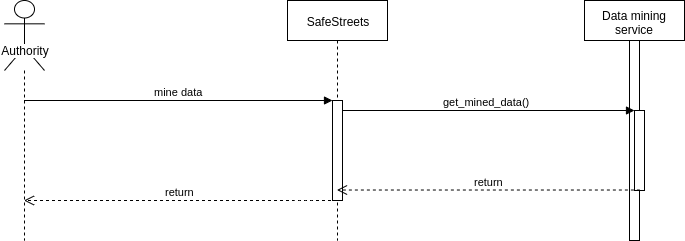
\includegraphics[width=\linewidth]{UML/Data_mining_sequence_diagram.png}
		\caption{Data mining: sequence diagram}
	\end{figure}

		\begin{table} [H]
		\begin{center}
		\caption{Issuing tickets}
		\begin{tabular}{|c|p{8cm}|}
			\hline
			Actor			&	Authorities\\
			\hline
			Entry condition	&	\begin{itemize}[noitemsep,topsep=0pt]
									\item The user is signed in into the application
								\end{itemize}\\
			\hline
			 Events flow		&	\begin{enumerate}[noitemsep,topsep=0pt]
									\item User see all the recieved photos from 
									citizens by order
									\item User clicks on one of them to analize the details
									\item Decide to choose Issuing the ticket or Ignore it 
									(for some reason such as this licence plate belongs to 
									some justified people)
									\item \textbf{Provide infos about the ticket 
									(ex: how much money}
								\end{enumerate}\\
			\hline
			Exit condition	&	\begin{itemize}[noitemsep,topsep=0pt]
									\item The authority releases a ticket for 
									the choosen violation
									\item If the owner of the plate which recived 
									the ticket is a SefeStreets user, he's notified 
									of the ticket
								\end{itemize}\\
			\hline
			Exeption			&	\begin{itemize}[noitemsep,topsep=0pt]
									\item Server is unreachable
									\item Violation is discarded
								\end{itemize}\\
			\hline
		\end{tabular}
		\end{center}
		\end{table} 
		
	\begin{figure}
		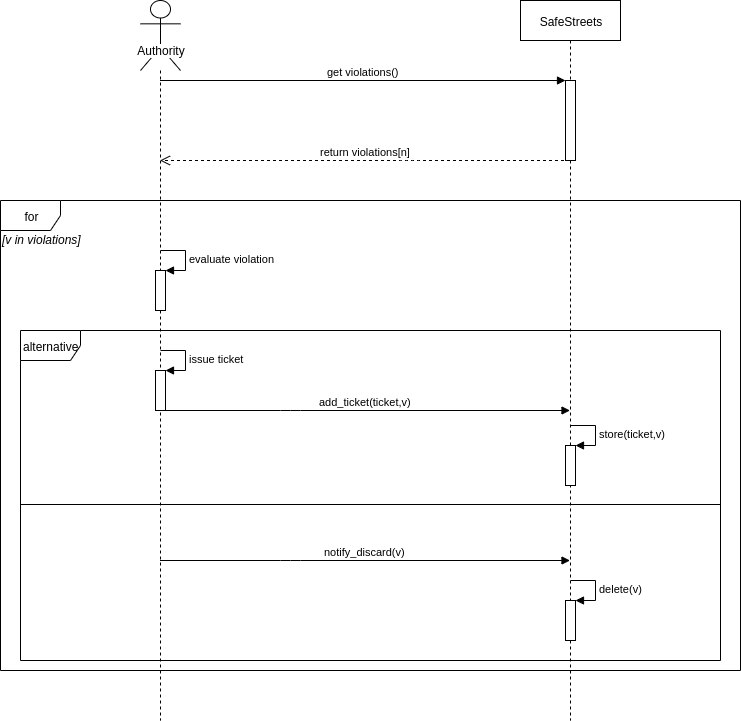
\includegraphics[width=\linewidth]{UML/Issue_ticket_sequence_diagram.png}
		\caption{Issue ticket: sequence diagram}
	\end{figure}
		
	\newpage
	
	\subsection{Product functions}
	The main functions of the system follows (lines in parenthesis are outside the system domain but are inserted for completeness):
		\paragraph{Violation notification}
			This is the core function of the system, exploited by the citizens.
			This function can be divided in 3 parts:
				\begin{itemize}
					\item \textbf{Data gathering}
					When the user spots the violation and with the help of its phone fills all the data (hopefully many will be gathered automatically) and sends them to the server
					\item \textbf{Elaboration}
					When the data are recived by our server the integrity of the data is checked; then a computer vision algorithm elaborates the plate. Finally, all the encoded data are stored to the database.
					\item \textbf{Acknowledgment}
					After the elaboration, the user recives a message confirming everything was ok, or asking more data if something went wrong during the elaboration.
				\end{itemize}
				
		\paragraph{Violation examination}
			This is the way the system could deeply influence the world. This function, exploited by recognized authorities, is the first step for automatically releasing tickets (which is not doable as pointed out by \ref{C_noAutoTickets}. In particular, the authority will:
			\begin{itemize}
				\item Access the server from its interface
				\item Retrieve data about violation
				\item Check the data
				\item (If data are correct, decide if a ticket can be created and in case create it)
			\end{itemize}
			In case a ticket is issued to a SafeStreets user, he/she will be notified about it, and will recive informations about the violation and the fee of the ticket itself.
		
		\paragraph{Statistics}
			This funciton can be exploited by any user. Basically, it concerns the displaying of statistics about violations in a graphic, map-based \textbf{structure}. It is composed by the following steps:
			\begin{itemize}
				\item A data-mining service runs on our servers, mining the database
				\item Data are aggregated by some rule
				\item Aggregated data are ordered
				\item The ordered aggregated data is displayed in a propter way
			\end{itemize}
			The way data are aggregated, ordered and displayed are now listed:
				\subparagraph{Map-based} Data are displayed in a map marking the streets of the city with different colors, one for each identified "class of risk". A street is identified with a class of risk based on the number of violations in that streets in the last 3 months.
				\subparagraph{List of vehicles} Veichles are sorted by number of violations, the ones with the highest number comes first. Depending on privacy laws, a picture of the vehicle taken from the pictures of violations, with the plate hidden, could be displayed
				\subparagraph{City data} General statistics about the violations in the city can be viewed from authorities to decide about \textbf{SOMETHING TO DO}
				
		\begin{figure}[H]
			\centering
			\def\svgwidth{\columnwidth}
			\input{Images/Notify_Violation_Class_Diagram.pdf_tex}
		\caption{High level class diagram for violation notification and examination}
		\end{figure}
				
		\begin{figure}[H]
			\centering
			\def\svgwidth{\columnwidth}
			\input{Images/Statistics_class_diagram.pdf_tex}
		\caption{High level class diagram for Statistic production and presentation}
		\end{figure}
			
	
	\subsection{Assumptions, dependencies and constraints}
	
	\paragraph{Assumptions:}
		\begin{enumerate}[label=\enum{A}]
			\item \label{A_disjPlates} Different cars always have different plates
			\item \label{A_Single plate}Each car exactly has 1 plate
			\item \label{A_singleOwner}No car is owned by more than 1 person
			\item \label{A_accessiblePermissions}Every auth will have access to any permission released by any other auth. SafeStreets will have access too.
			\item \label{A_noGeneratedModifiedNotif}Every modified notification has a corresponding non-modified one (even only theoretical)
			\item \label{A_newNotificationsAreNotModified}When a notification is created it is unmodified. Modifications can happen later, generating a new notification (see \ref{A_noGeneratedModifiedNotif})
			\item \label{A_authsNotClairvoyants}If a notification is not stored then no auth can see it and therefore no ticket can be released for that notification
		\end{enumerate}
	
	\paragraph{Constraints:}
		\begin{enumerate}[label=\enum{C}]
			\item The authorities will not be able to register automatically to the service. For authentication, they'll be verified and added by an administrator of the system
			\item \label{C_noAutoTickets}Due to italian law, the system won't be able to automatically produce tickets
		\end{enumerate}
	
\newpage
\section{Specific Requirements} \textit{Here we include more details on all the aspects in Section 2 if they can be used for the development team}

		\subsubsection{Scenarios}
		
			\begin{enumerate}[label=\enum{S}]
				\item \label{S_The man, the street and the monstertruck}
				Mario is walking down the street when he comes to a cross. He would like to \textbf{cross the cross} staying on the pedestrian lines, but a monstertruck decided to park over there. So Mario needs to walk around the truck and through the street (cars are driving fast), but at least he can take a little revenge by taking out his mobile phone, opening the SafeStreets application and take a picture of the plate of the truck. The application automatically acquires data on time and position using the gps and sends the data to SafeStreets' server. In a second, Mario is notified that the violation has been saved and will be avilable for the police.
Mario now knows the crazy-minded driver will pay what he deserves! (like some fines)
				\item \label{S_Prevent is better than healing}Luigi is late for work. He cannot find any parking, and is thinking about parking on the bycicle line. He's about to do that, when he suddently remembers that nowaday anyone could signal his infractions with SafeStreets. So he decides to keep searching for a proper parking, and granny Maria can take her daily ride on her bycicle!
			\end{enumerate}

\newpage
	\subsection{External Interface Requirements}
		These requirements come from the needing to communicate to the local police to submit notifications and gather ticket statistics, and to reduce the project cost by outsourcing.
		
		\subsubsection{User Interfaces}
		
			\begin{figure}[H]
				\centering
				\begin{subfigure}[H]{0.25\linewidth}
					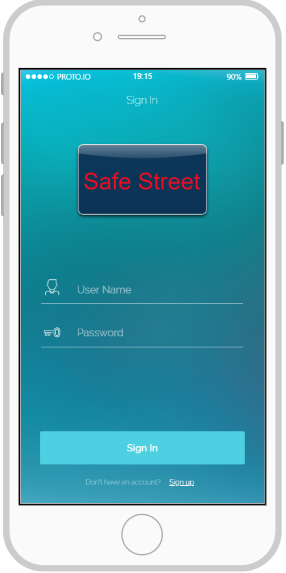
\includegraphics[width=\linewidth]{Images/Sign_In.png}
					\caption{Sign in}
				\end{subfigure}	
				\begin{subfigure}[H]{0.25\linewidth}
					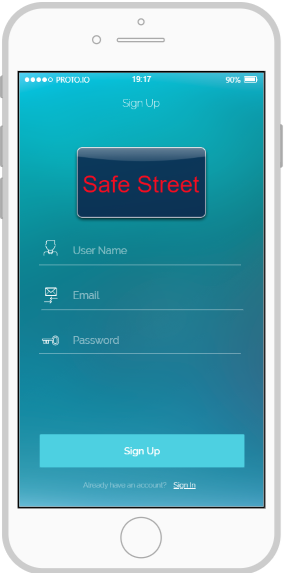
\includegraphics[width=\linewidth]{Images/Sign_Up.png}
					\caption{Sign up}
				\end{subfigure}
				\begin{subfigure}[H]{0.25\linewidth}
					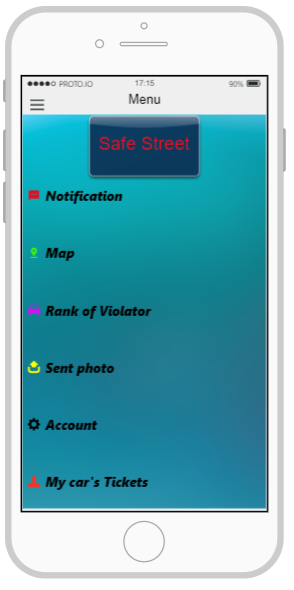
\includegraphics[width=\linewidth]{Images/Menu.png}
					\caption{Menu}
				\end{subfigure}
				\begin{subfigure}[H]{0.25\linewidth}
					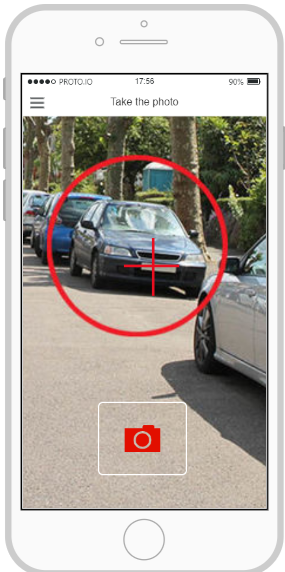
\includegraphics[width=\linewidth]{Images/Camera.png}
					\caption{Menu}
				\end{subfigure}
				\begin{subfigure}[H]{0.25\linewidth}
					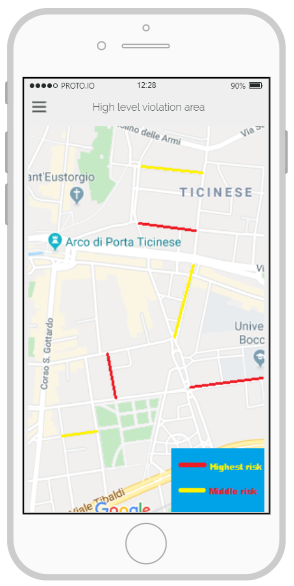
\includegraphics[width=\linewidth]{Images/Maps.png}
					\caption{Menu}
				\end{subfigure}
				\begin{subfigure}[H]{0.25\linewidth}
					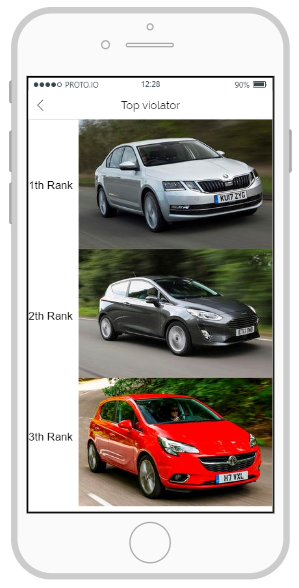
\includegraphics[width=\linewidth]{Images/Top_Violators.png}
					\caption{Menu}
				\end{subfigure}
			\end{figure}				
			\newpage	
		
			\begin{enumerate}[label=\enum{UI}]
				\item A graphical user interface should be provided to the auths to allow them to retrive data manually. It could be web-based or desktop-based.
				\item \label{UI_mobileApp}The citizen's user interface should be a mobile application to both be able to ensure mobility and security, being able to control the dataflow.
			\end{enumerate}
			
		\subsubsection{Software Interfaces}
			\begin{enumerate}[label=\enum{SW}]
				\item An api should be produced to allow auth's servers to access data programmatically
				\item An external api should be used to manage the map-based displaying of statistics
			\end{enumerate}
			
	\subsection{Functional Requirements} \textit{Definition of use case diagrams, usa cases and associated sequence/activity diagrams, and mapping on requirements}
			
		\subsubsection{Requirements}
		
			\begin{enumerate}[label=\enum{R}]
				\item \label{R_storeTickets}Requires the authorities to give SafeStreets access to the tickets they emitted using SafeStreets' data
				\item \label{R_autoPlate}Automatically extract the plate number of the car from the photo, ignoring cars in the background if present
				\item \label{R_unalteredData}Ensure no data is altered from the insertion to the eventual storage
				\item \label{R_dataGather}For each data to insert, if the  user's device has a sensor to collect thatkind of data, that sensor should be used instead of manual insertion (example: GPS). Otherwise it will be possible to insert it by hand.
				\item \label{R_notifyUser}The system should notify the user when his notification has been processed correctly, or ask for more datailed data (example: a more focused picture) if needed.
				\item \label{R_fullData}If a notification is missing any needed data, the client application will prevent the user from sending it
				\item \label{R_modifiedNotStored}No modified notification will be stored by SafeStreets
				\item \label{R_validPermissionNotStored}If a violation is invalidated by a permission, it won't be stored
				\item \label{R_legitNotificationsAlwaysStored}All notifications which are not modified and neither covered by a permission will be saved
			\end{enumerate}
				
	\subsection{Performance requirements}
		\begin{enumerate}[label=\enum{P}]
			\item The notification should be sent to the server as soon as possible. It should be recived and elaborated as soon as internet and the server's speed allows to match almost-real-time speed
			\item The quality of the photo should be at most XYZ (to reduce overload on network and server) but at least PQR (to enable automatic recognition).
		\end{enumerate}
		
	\subsection{Design Constraints}
	
		\subsubsection{Hardware limitations} 
			\begin{enumerate}[label=\enum{SW}]
				\item The auth's hardware will require an internet connection to access the data.
				\item The cit's device will have to be a smartphone for the reasons explained in \ref{UI_mobileApp}
			\end{enumerate}					
		
		\subsubsection{Any other constraint} 
			\begin{enumerate}[label=\enum{OT}]
				\item The citizen's device should be checked to be trustable, and rooted devices should be blocked (as they could change the app behaviour and submit altered photos)
			\end{enumerate}		
		
	\subsection{Software system attributes}
	
		\subsubsection{Reliability}
			The only critical part of the system is the one concerning data mining, as people could exploit it to decide about it's daily routine. For this reason, it's recommended to make the result of the mining (old ones if needed) more available than the rest of the system.
			In addiction, the system must avoid to generate fake notifications because of system faults to prevent innocent people from getting an unfair ticket.
			
		\subsubsection{Availability}
			As the system does not concern life-critical events, we think an availability of 99\% of the time should be enought to ensure a good experience for both cits and auths.
			
		\subsubsection{Security}
			\begin{list}{-}{}
				\item Transmit data encrypted to prevent alteration in the network
				\item Only allow auths to access non-aggregated data
			\end{list}
			
		\subsubsection{Maintainability}
			Maintainability is not a crucial issue as no updates are planned for the system.
			
		\subsubsection{Portability}
			Portability is a crucial aspect of the system, at least on the citizen's side: it is needed to allow them to submit a notification as they spot a violation. For this reason, the cit's client should be avaiable on as most mobile devices as possible.
			
	\subsection{Traceability matrix}
		\begin{table}[H]
			\begin{center}
				\caption{Traceability matrix}
				\label{Trace matrix}
				\begin{tabular}{c|c|c}
					\textbf{Goal ID} & \textbf{Req ID} & \textbf{Usecase ID}\\
					\hline
					\ref{G_realTime} 	& \ref{R_autoPlate}	& \ref{S_The man, the street and the monstertruck}\\
										&\ref{R_dataGather}	&\\
										&\ref{R_notifyUser}	&\\
					\hline
					\ref{G_allData} 	& \ref{R_dataGather} & \\
									& \ref{R_fullData} & \\
					\hline
					\ref{G_helpAuth}	&\ref{A_disjPlates}&\\
									&\ref{A_Single plate}&\\
									&\ref{A_singleOwner}&\\
									&\ref{A_accessiblePermissions}&\\
									&\ref{A_noGeneratedModifiedNotif}&\\
									&\ref{A_newNotificationsAreNotModified}&\\
									&\ref{R_autoPlate}&\\
									&\ref{R_unalteredData}&\\
									&\ref{R_fullData}&\\
					\hline
					\ref{G_discardAltered}	&\ref{A_noGeneratedModifiedNotif}&\\
											&\ref{A_newNotificationsAreNotModified}&\\
											&\ref{R_unalteredData}&\\
											&\ref{R_dataGather}&\\
											&\ref{R_fullData}&\\
											
					\hline
					\ref{G_respectPermissions}	&\ref{A_disjPlates}&\\
												&\ref{A_Single plate}&\\
												&\ref{A_accessiblePermissions}&\\
												&\ref{R_autoPlate}&\\
					\hline
					\ref{G_storeFine}	&\ref{A_disjPlates}&\\
										&\ref{A_Single plate}&\\
										&\ref{A_accessiblePermissions}&\\
					\hline
					\ref{G_statistics}	&\ref{R_storeTickets}\\
										&\ref{R_dataGather}&\\
										&\ref{R_fullData}&\\
										
				\end{tabular}
			\end{center}
		\end{table}
		
\newpage
\section{Formal analysis using alloy} \textit{This section should include a brief presentation of the main objectives driving the formal modeling activity, as well as a description of the model itself, what can be proved with it, and why what is proved is important given the problem at hand. To show the soundness and correctness of the model, this section can show some worlds obtained by running it, and/or the results of the checks performed on meaningful assertions}
	\paragraph{}The signatures are omitted in the document as they reflect the entities 				desctibes in section \ref{definitions}, plus some "enumerations". The goals we were able to define in Alloy are \ref{G_discardAltered},\ref{G_respectPermissions} and \ref{G_storeFine}.
	There was no need to check \ref{G_statistics} and \ref{G_allData} as they can be satisfied 	by an equal requirement
	\paragraph{}The assumptions we were able to define are \ref{A_disjPlates}, \ref{A_Single plate}, \ref{A_singleOwner}, \ref{A_accessiblePermissions}. Please note not all of them has been expressed by facts as some was already expressed by multiplicity in the signatures.
	\lstinputlisting[language=alloy]{Alloy/Alloy.als}
	
\newpage
\section{Effort spent} \textit{In this section you will include information about the number of hours each group member has worked for this document}

	\paragraph{Matteo Secco} 
		\begin{list}{-}{}
			\item October 16: Introduction and Scope. 30m
			\item October 16: Definitions. 15m.
			\item October 23: Scenarios and goals. toghether. 1h
			\item October 24: Update goals, assumptions, alloy skeleton. 2h
			\item October 24: Teamwork. 2h
			\item October 27: Traceabiity matrix and related. 1.30h
			\item October 28: modify some Tasks toghether. 1h
			\item October 30: Design fixes, product functions. 1.30h
			\item October 30: Alloy. 1h
			\item November 2: Alloy. 1h
			\item November 3: Use-cases. 1h
			\item November 3: Alloy. 2h
			\item November 6: Alloy: 1h
			\item November 6: UML: 1h
			\item November 7: Phenomena. 30m
		\end{list}
		
	\paragraph{Rahbari}
		\begin{list}{-}{}
			\item October 23: Scenarios and goals. toghether. 1h
			\item October 24: Teamwork. 2h
			\item October 27: Use case diagram,product prospective 2h
			\item October 28: Modify some Tasks toghether. 1h
			\item October 30: use case table. 1h
			\item November 3: finishing all the use case tables 2h
			\item November8: working on Sequence Diagram 3h
		\end{list}
\section{References}
\end{document}
